\section{Reproducing the results}
\label{app:repro}

The paper repository (\href{https://github.com/kylemcdonald/shufflesnap-paper}{\nolinkurl{github.com/kylemcdonald/shufflesnap-paper}}) contains every script, raw result, and figure
source. The implementation is a separate repository (\href{https://github.com/kylemcdonald/shufflesnap}{\nolinkurl{github.com/kylemcdonald/shufflesnap}}); the benchmarked code is
identical, apart from its version string, to release 0.4.0 on PyPI
(\texttt{pip install shufflesnap}). Starting from a checkout of both side by side:
{\small
\begin{verbatim}
pip install ./shufflesnap[exact]   # C++ build, ~2 s
pip install -r shufflesnap-paper/requirements.txt
cd shufflesnap-paper
python experiments/make_embeddings.py mnist fashion   # UMAP, fixed seed
python experiments/references_all.py 6                # certified optima (parallel)
bash experiments/make_frozen_snapshot.sh              # v0.4.0 snapshot under test
bash experiments/run_all.sh                           # all benchmarks, sequential
bash experiments/run_swap.sh                          # RasterFairy's swap optimizer
python experiments/small_exactness.py                 # small-N exactness table
python experiments/dev_ablation.py                    # development-set search
python experiments/seed_study.py                      # spread over inputs and starts
python experiments/seed_study_report.py
python experiments/make_figures.py all && python experiments/make_tables.py
python experiments/fig_method.py; python experiments/fig_failures.py
python experiments/fig_reference.py                   # annotated reference
python experiments/fig_visual.py mnist; python experiments/fig_visual.py fashion
python experiments/fig_masks.py
cd paper && tectonic main.tex
\end{verbatim}
}
Raw results are JSON lines in \texttt{results/raw/}: one record per run, holding the
full run specification, timings, memory, validity check, cost, displacement statistics,
and the software environment (library versions, commit hashes of the comparator
repositories). Certified optima are cached in \texttt{results/reference/} with their
lower bound and gap. The lab notebook \texttt{notebook/LOG.md} records decisions and
negative results in the order they happened.

\paragraph{Timing boundary (summary).} A timed run is one call of a method adapter in a fresh
process, after a warm-up call on a 256-point instance. It includes method-specific
preprocessing and excludes instance generation, the shared normalization, and
validation. Peak memory is the rise of peak RSS during the call.

% Generated by experiments/fig_reference.py from paper/reference.py; do not edit.
\begin{landscape}
\section{A serial reference implementation}
\label{app:reference}

\noindent\begin{minipage}[t]{0.405\linewidth}\vspace{0pt}\raggedright
{\small This is the complete algorithm: the file \texttt{shufflesnap/reference.py} from the
package, split into its parts, each beside a diagram computed with its code. Without exact
ties it returns the same assignment as the compiled kernel; the package's tests check this
for every preset on six kinds of target, from an exact-fit square to surplus cells and a
random mask. The kernel adds threads, skips windows whose cells have not changed (which does
not change the result) and an optional time budget. Points are in grid units: cell $(x,y)$
has its center at $(x,y)$.\par}
\end{minipage}\hfill
\begin{minipage}[t]{0.565\linewidth}\vspace{0pt}
\lstinputlisting[firstline=1,lastline=12,firstnumber=1,numbers=left,numberstyle=\tiny\color{black!45},numbersep=6pt,frame=none,xleftmargin=1.6em,aboveskip=0pt,belowskip=0pt]{reference.py}
\end{minipage}

\vspace{1.4em}
\noindent\begin{minipage}[t]{0.405\linewidth}\vspace{0pt}\raggedright
\textbf{The schedule.}\par\smallskip
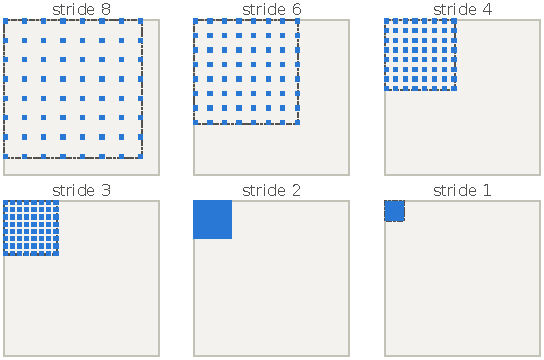
\includegraphics[width=\linewidth]{figures/fig_ref_schedule}\par\smallskip
{\small A window always holds $w\times w$ cells, but at stride $s$ they lie $s$ cells apart, so
it spans $(w-1)s+1$ cells per axis (dashed). The first stride is the smallest power of two
with $ws\ge L$, so the first windows reach across the axis; each later stride is the last one
divided by \texttt{ratio} and rounded. Each axis has its own strides, and the shorter axis
waits at 1. Drawn: one window of the default preset ($w=8$) on a $64\times64$ grid at every
stride.\par}
\end{minipage}\hfill
\begin{minipage}[t]{0.565\linewidth}\vspace{0pt}
\lstinputlisting[firstline=15,lastline=34,firstnumber=15,numbers=left,numberstyle=\tiny\color{black!45},numbersep=6pt,frame=none,xleftmargin=1.6em,aboveskip=0pt,belowskip=0pt]{reference.py}
\end{minipage}

\clearpage
\noindent\begin{minipage}[t]{0.405\linewidth}\vspace{0pt}\raggedright
\textbf{The windows of one tiling.}\par\smallskip
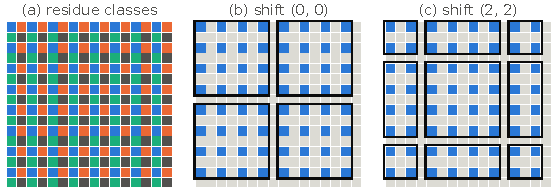
\includegraphics[width=\linewidth]{figures/fig_ref_windows}\par\smallskip
{\small At stride $(s_x,s_y)$ the cells fall into $s_xs_y$ residue classes $(x \bmod s_x,\,
y \bmod s_y)$ (a). In its class, cell $x$ is lattice column $x /\!/ s_x$, and tiles of $w$
lattice columns start at column \texttt{ox}. A window is the set of cells that share a class
and a tile (b, boxes). The four tilings of a round shift the tiles by half a window (c). Edge
windows are smaller, and masked cells never appear. Drawn with $w=4$, stride 2, class
$(0,0)$.\par}
\end{minipage}\hfill
\begin{minipage}[t]{0.565\linewidth}\vspace{0pt}
\lstinputlisting[firstline=37,lastline=44,firstnumber=37,numbers=left,numberstyle=\tiny\color{black!45},numbersep=6pt,frame=none,xleftmargin=1.6em,aboveskip=0pt,belowskip=0pt]{reference.py}
\end{minipage}

\vspace{1.4em}
\noindent\begin{minipage}[t]{0.405\linewidth}\vspace{0pt}\raggedright
\textbf{One window.}\par\smallskip
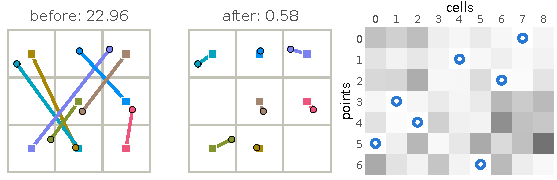
\includegraphics[width=\linewidth]{figures/fig_ref_solve}\par\smallskip
{\small The window's points are reassigned among all of its cells, empty ones included, by an
exact linear assignment on squared distances. The result is kept only if it lowers the
window's cost by more than a relative \texttt{tol}, so the cost never rises and ties cannot
cycle. \texttt{pos} gives each point's cell and \texttt{occ} each cell's point. Drawn: seven
points in a $3\times3$ window before and after, with summed squared distances, and the cost
matrix with the chosen entries.\par}
\end{minipage}\hfill
\begin{minipage}[t]{0.565\linewidth}\vspace{0pt}
\lstinputlisting[firstline=47,lastline=59,firstnumber=47,numbers=left,numberstyle=\tiny\color{black!45},numbersep=6pt,frame=none,xleftmargin=1.6em,aboveskip=0pt,belowskip=0pt]{reference.py}
\end{minipage}

\clearpage
\noindent\begin{minipage}[t]{0.405\linewidth}\vspace{0pt}\raggedright
\textbf{The whole method.}\par\smallskip
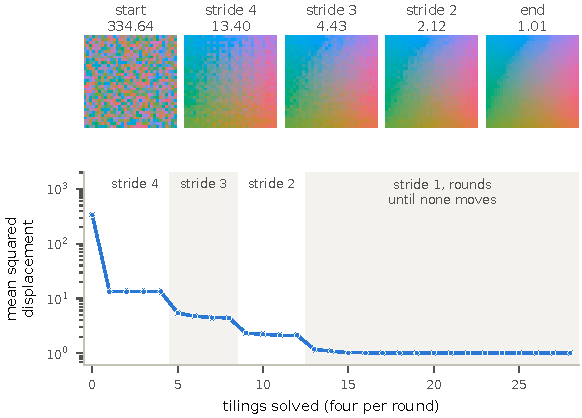
\includegraphics[width=\linewidth]{figures/fig_ref_snap}\par\smallskip
{\small The cells are the mask's usable entries in row-major order, and point $i$ starts in a
random cell \texttt{pos[i]}. A round solves the windows of the four tilings in turn. Each
coarse stage runs one round; then stride-1 rounds repeat until one moves nothing, a fixed
point of every window but not a proof of optimality. Drawn: 1{,}024 uniform points on a
$32\times32$ grid, colored by input position, after the start, each
coarse stage and the end (top), and the mean squared displacement in cells$^2$ after every
tiling (bottom): each stride halves it or better, and the last stride-1 round moves
nothing.\par}
\end{minipage}\hfill
\begin{minipage}[t]{0.565\linewidth}\vspace{0pt}
\lstinputlisting[firstline=62,lastline=83,firstnumber=62,numbers=left,numberstyle=\tiny\color{black!45},numbersep=6pt,frame=none,xleftmargin=1.6em,aboveskip=0pt,belowskip=0pt]{reference.py}
\end{minipage}
\end{landscape}


\section{Additional tables}
\label{app:tables}

\begin{table}[tbp]
\centering\scriptsize
\setlength{\tabcolsep}{3.2pt}
\caption{Absolute excess over the certified optimum, in cells$^2$ per point, at $N=100{,}000$
(same runs as Table~\ref{tab:main}). ``Optimum'' is the certified optimal mean squared
displacement. Relative and absolute excess tell different stories on the heavy-tailed
input, where outliers dominate the optimum.}
\label{tab:abs}
\resizebox{\linewidth}{!}{\begin{tabular}{lrrrrrrrrr}
\toprule
distribution & optimum & SS fast & BSP 16 & SS bal. & BSP 64 & SS qual. & RF master & RF PyPI & Bisect. \\
\midrule
uniform & 1.80 & 0.045 & 0.80 & 0.015 & 0.58 & 0.008 & 0.80 & 1.10 & 1.81 \\
Gaussian & 6501 & 0.030 & 3.61 & 0.011 & 2.60 & 0.005 & 0.38 & 0.66 & 1.17 \\
Gaussian mixture & 4440 & 0.58 & 252 & 0.11 & 167 & 0.010 & 751 & 752 & 554 \\
90/10 clusters & 8743 & 4.34 & 2.77 & 1.01 & 1.66 & 0.079 & 102 & 101 & 49.9 \\
ring & 1731 & 0.081 & 20.1 & 0.022 & 16.5 & 0.008 & 710 & 710 & 697 \\
spiral & 1338 & 0.29 & 133 & 0.055 & 108 & 0.015 & 366 & 367 & 460 \\
checkerboard & 32.1 & 0.041 & 16.0 & 0.018 & 11.6 & 0.006 & 137 & 137 & 145 \\
heavy tails & 32818 & 0.009 & 0.019 & 0.007 & 0.012 & 0.005 & 0.018 & 0.070 & 0.059 \\
duplicates & 4136 & 5.88 & 491 & 1.45 & 228 & 0.47 & 2034 & 2035 & 1645 \\
near-line & 9876 & 0.98 & 0.81 & 0.21 & 0.20 & 0.033 & 1912 & 1912 & 1884 \\
\bottomrule
\end{tabular}
}
\end{table}

\begin{table}[tbp]
\centering\scriptsize
\setlength{\tabcolsep}{3.2pt}
\caption{As Table~\ref{tab:main}, at $N=10{,}000$. Here the dense SciPy solver is feasible; the
last column gives its time on instance seed 1 (it returns the same optimum as the
certified solver).}
\label{tab:main10k}
\resizebox{\linewidth}{!}{\begin{tabular}{lrrrrrrrrrr}
\toprule
distribution & SS fast & BSP 16 & SS bal. & BSP 64 & SS qual. & RF master & RF PyPI & Bisect. & exact (s) & dense (s) \\
\midrule
uniform & 2.34 & 27.6 & 0.69 & 17.9 & 0.28 & 31.8 & 82.4 & 86.2 & 0.53 & 10.8 \\
Gaussian & 0.003 & 0.13 & 0.001 & 0.093 & $<$0.001 & 0.040 & 0.14 & 0.15 & 1.31 & 205 \\
Gaussian mixture & 0.014 & 3.78 & 0.004 & 2.54 & $<$0.001 & 38.7 & 39.7 & 13.1 & 2.05 & 176 \\
90/10 clusters & 0.037 & 0.13 & 0.011 & 0.049 & 0.001 & 1.32 & 1.47 & 0.66 & 2.91 & 227 \\
ring & 0.018 & 3.78 & 0.007 & 1.56 & 0.005 & 40.5 & 41.6 & 39.4 & 1.92 & 104 \\
spiral & 0.036 & 10.3 & 0.013 & 7.30 & 0.005 & 24.6 & 29.9 & 31.9 & 2.29 & 84.9 \\
checkerboard & 0.72 & 55.4 & 0.28 & 44.8 & 0.090 & 271.4 & 260.7 & 265.2 & 0.53 & 15.9 \\
heavy tails & $<$0.001 & 0.005 & $<$0.001 & 0.003 & $<$0.001 & $<$0.001 & 0.002 & 0.003 & 3.21 & 352 \\
duplicates & 0.15 & 12.0 & 0.045 & 4.97 & 0.014 & 57.6 & 58.0 & 36.6 & 0.97 & 126 \\
near-line & 0.012 & 0.027 & 0.003 & 0.007 & $<$0.001 & 19.4 & 19.8 & 19.5 & 6.92 & 246 \\
\midrule
\emph{median time (s)} & 0.057 & 0.063 & 0.15 & 0.25 & 0.42 & 0.22 & 0.029 & 0.003 & 1.99 & 151 \\
\bottomrule
\end{tabular}
}
\end{table}

\begin{table}[tbp]
\centering\scriptsize
\setlength{\tabcolsep}{3.2pt}
\caption{As Table~\ref{tab:main}, at $N=50{,}000$.}
\label{tab:main50k}
\resizebox{\linewidth}{!}{\begin{tabular}{lrrrrrrrrrr}
\toprule
distribution & SS base & SS fast & SS bal. & SS qual. & BSP 16 & BSP 64 & RF master & RF PyPI & Bisect. & exact (s) \\
\midrule
uniform & 3.61 & 2.24 & 1.20 & 0.48 & 45.5 & 36.8 & 40.4 & 65.4 & 114.2 & 6.82 \\
Gaussian & $<$0.001 & $<$0.001 & $<$0.001 & $<$0.001 & 0.056 & 0.039 & 0.009 & 0.018 & 0.031 & 38.4 \\
Gaussian mixture & 0.012 & 0.008 & 0.001 & $<$0.001 & 5.47 & 3.83 & 38.2 & 38.2 & 14.6 & 47.6 \\
90/10 clusters & 0.031 & 0.026 & 0.005 & $<$0.001 & 0.049 & 0.025 & 1.21 & 1.22 & 0.86 & 65.1 \\
ring & 0.017 & 0.004 & 0.002 & $<$0.001 & 2.15 & 0.59 & 41.1 & 41.1 & 42.2 & 37.6 \\
spiral & 0.025 & 0.014 & 0.006 & 0.002 & 11.4 & 7.74 & 27.3 & 27.4 & 25.0 & 43.1 \\
checkerboard & 0.29 & 0.16 & 0.085 & 0.035 & 81.6 & 69.4 & 398.0 & 400.1 & 423.4 & 14.4 \\
heavy tails & $<$0.001 & $<$0.001 & $<$0.001 & $<$0.001 & $<$0.001 & $<$0.001 & $<$0.001 & $<$0.001 & $<$0.001 & 92.1 \\
duplicates & 0.11 & 0.083 & 0.038 & 0.013 & 13.8 & 4.91 & 58.6 & 58.6 & 39.7 & 151 \\
near-line & 0.007 & 0.002 & $<$0.001 & $<$0.001 & 0.028 & 0.003 & 19.7 & 19.7 & 19.5 & 77.9 \\
jittered lattice & 24.5 & 17.3 & 13.1 & 6.91 & 59.4 & 41.2 & 12.1 & 27.7 & 205.6 & 2.87 \\
\midrule
\emph{median time (s)} & 2.26 & 3.04 & 6.95 & 22.6 & 0.34 & 1.36 & 1.45 & 12.4 & 0.016 & 43.1 \\
\bottomrule
\end{tabular}
}
\end{table}

\begin{table}[tbp]
\centering\scriptsize
\setlength{\tabcolsep}{3.2pt}
\caption{RasterFairy's swap optimizer (upstream \texttt{rfoptimizer.py}) at $N=2{,}500$
($50\times50$ grid), mean excess over the certified optimum (\%) over instance seeds 1--3,
one thread. RF is RasterFairy upstream; the next four columns run the swap optimizer from its
layout for $10^4$ to $10^7$ iterations, and the last one from a random permutation, as in
upstream's demo. \textsuperscript{a}: timed on another physical core (seed 1) or on five
others in parallel (seeds 2--3). The dense SciPy solver returns the optimum in a median of
2.7\,s.}
\label{tab:swap}
\resizebox{\linewidth}{!}{\begin{tabular}{lrrrrrrrrrrr}
\toprule
 & & & & & & & \multicolumn{4}{c}{RF + swap optimizer} & \\
\cmidrule(lr){8-11}
distribution & SS fast & SS bal. & SS qual. & BSP 16 & BSP 64 & RF & $10^4$ & $10^5$ & $10^6$ & $10^7$\textsuperscript{a} & rand.\ $10^6$ \\
\midrule
uniform & 1.56 & 1.05 & 0.30 & 26.8 & 19.3 & 16.6 & 16.6 & 16.2 & 15.2 & 13.9 & 6320 \\
Gaussian & 0.012 & 0.006 & 0.001 & 0.22 & 0.15 & 0.11 & 0.11 & 0.11 & 0.11 & 0.100 & 29.5 \\
Gaussian mixture & 0.033 & 0.012 & 0.002 & 6.06 & 3.58 & 38.3 & 33.7 & 28.7 & 18.1 & 10.4 & 39.3 \\
90/10 clusters & 0.048 & 0.013 & 0.005 & 0.29 & 0.16 & 1.20 & 1.16 & 1.06 & 0.82 & 0.50 & 17.1 \\
ring & 0.053 & 0.018 & 0.004 & 2.95 & 2.24 & 35.9 & 35.3 & 33.2 & 21.5 & 12.3 & 101.7 \\
spiral & 0.13 & 0.036 & 0.012 & 9.64 & 5.53 & 10.4 & 10.3 & 9.97 & 8.82 & 7.16 & 140.0 \\
checkerboard & 1.15 & 0.43 & 0.33 & 51.2 & 36.1 & 56.3 & 56.0 & 52.5 & 45.1 & 33.6 & 4346 \\
heavy tails & $<$0.001 & $<$0.001 & $<$0.001 & 0.006 & 0.004 & 0.003 & 0.003 & 0.003 & 0.002 & 0.002 & 0.43 \\
duplicates & 0.17 & 0.050 & 0.015 & 9.03 & 6.77 & 55.6 & 54.0 & 48.7 & 36.7 & 30.2 & 50.1 \\
near-line & 0.015 & 0.004 & 0.002 & 0.070 & 0.020 & 19.2 & 14.3 & 11.6 & 1.65 & 0.81 & 6.98 \\
\midrule
\emph{median time (s)} & 0.012 & 0.029 & 0.071 & 0.015 & 0.059 & 0.051 & 0.75 & 6.44 & 63.3 & 613 & 61.7 \\
\bottomrule
\end{tabular}
}
\end{table}

\begin{figure}[tbp]
  \centering
  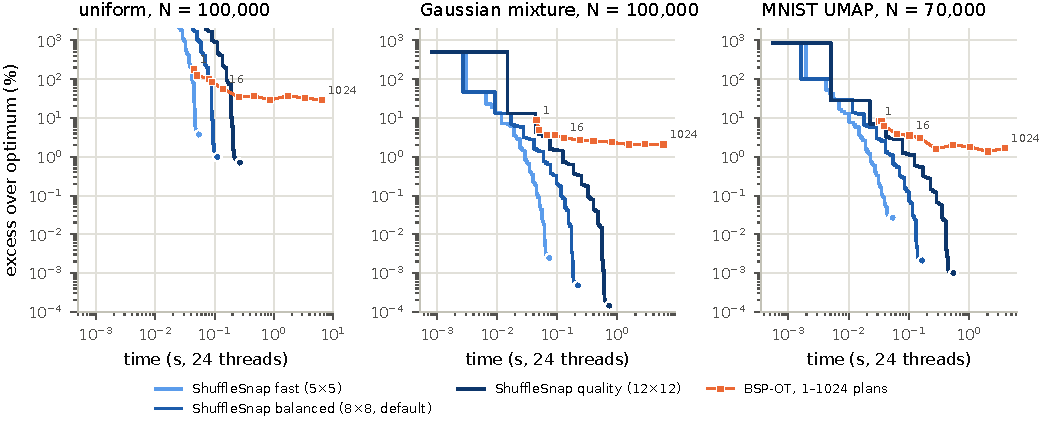
\includegraphics[width=\linewidth]{figures/fig_anytime_t24.pdf}
  \caption{As Figure~\ref{fig:anytime}, with 24 threads for \ShuffleSnap\ and BSP-OT
  (RasterFairy is single-threaded).}
  \label{fig:anytime24}
\end{figure}

\begin{table}[tbp]
\centering\scriptsize
\caption{All held-out ablations (24 threads): mean excess over the certified optimum (\%) and
median time (s) over instance seeds 1--3. Each row changes one setting of the default
($8\times8$ windows, stride ratio $\sqrt2$, four tilings, random start, one round per level,
geometric window solver, unchanged windows skipped, automatic start stride).}
\label{tab:ablation}
\resizebox{\linewidth}{!}{\begin{tabular}{llrrrrrr}
\toprule
change & setting & \multicolumn{2}{c}{uniform 100k} & \multicolumn{2}{c}{mixture 100k} & \multicolumn{2}{c}{MNIST 70k} \\
 & & excess \% & time (s) & excess \% & time (s) & excess \% & time (s) \\
\midrule
window side (ratio 2) & 3$\times$3 & 15.7 & 0.054 & 0.16 & 0.074 & 0.21 & 0.051 \\
 & 4$\times$4 & 6.36 & 0.072 & 0.035 & 0.12 & 0.079 & 0.084 \\
 & 5$\times$5 & 3.71 & 0.098 & 0.022 & 0.22 & 0.031 & 0.14 \\
 & 6$\times$6 & 2.51 & 0.13 & 0.011 & 0.37 & 0.015 & 0.24 \\
 & 7$\times$7 & 1.94 & 0.19 & 0.006 & 0.58 & 0.013 & 0.39 \\
 & 8$\times$8 & 1.52 & 0.25 & 0.004 & 0.87 & 0.004 & 0.59 \\
 & 10$\times$10 & 0.93 & 0.44 & 0.001 & 1.80 & 0.002 & 1.19 \\
 & 12$\times$12 & 0.54 & 0.68 & $<$0.001 & 3.16 & 0.001 & 2.12 \\
 & 16$\times$16 & 0.29 & 1.47 & $<$0.001 & 8.43 & $<$0.001 & 5.72 \\
\addlinespace
window side (ratio $\sqrt2$) & 4$\times$4 & 3.76 & 0.072 & 0.027 & 0.17 & 0.068 & 0.11 \\
 & 6$\times$6 & 1.50 & 0.14 & 0.008 & 0.53 & 0.010 & 0.35 \\
 & 8$\times$8 & 0.84 & 0.25 & 0.002 & 1.25 & 0.002 & 0.81 \\
 & 10$\times$10 & 0.54 & 0.42 & $<$0.001 & 2.49 & 0.002 & 1.55 \\
 & 12$\times$12 & 0.44 & 0.62 & $<$0.001 & 4.33 & $<$0.001 & 2.88 \\
 & 16$\times$16 & 0.19 & 1.32 & $<$0.001 & 11.1 & $<$0.001 & 7.78 \\
\addlinespace
stride ratio & 3 & 4.14 & 0.11 & 0.014 & 0.32 & 0.041 & 0.23 \\
 & 2 (baseline) & 2.51 & 0.13 & 0.011 & 0.37 & 0.015 & 0.25 \\
 & 1.68 & 1.99 & 0.13 & 0.007 & 0.43 & 0.011 & 0.28 \\
 & 1.41 & 1.50 & 0.14 & 0.008 & 0.53 & 0.010 & 0.35 \\
 & 1.19 & 1.58 & 0.17 & 0.009 & 0.80 & 0.013 & 0.50 \\
 & 1.1 & 1.93 & 0.20 & 0.009 & 1.04 & 0.018 & 0.64 \\
\addlinespace
start & random (baseline) & 2.51 & 0.14 & 0.011 & 0.37 & 0.015 & 0.24 \\
 & bisection & 29.9 & 0.16 & 0.21 & 0.73 & 0.14 & 0.33 \\
 & row sort & 22.9 & 0.13 & 0.042 & 1.02 & 0.12 & 0.41 \\
\addlinespace
rounds per level & 1 & 2.51 & 0.14 & 0.011 & 0.37 & 0.015 & 0.24 \\
 & 2 & 2.08 & 0.20 & 0.009 & 0.55 & 0.012 & 0.36 \\
 & 3 & 1.87 & 0.22 & 0.009 & 0.62 & 0.011 & 0.41 \\
\addlinespace
tilings per round & 1 & 21166 & 0.046 & 4.50 & 0.079 & 12.3 & 0.051 \\
 & 2 (diagonal) & 5.49 & 0.076 & 0.029 & 0.20 & 0.031 & 0.14 \\
 & 4 (baseline) & 2.51 & 0.13 & 0.011 & 0.36 & 0.015 & 0.24 \\
 & 9 & 1.86 & 0.27 & 0.006 & 0.76 & 0.008 & 0.51 \\
\addlinespace
first stride & automatic (baseline) & 2.51 & 0.12 & 0.011 & 0.35 & 0.015 & 0.24 \\
 & capped at 16 & 11.7 & 0.57 & 0.29 & 27.2 & 0.44 & 8.88 \\
 & capped at 8 & 10.9 & 0.95 & 0.27 & 29.1 & 0.54 & 11.5 \\
 & capped at 4 & 12.9 & 1.21 & 0.28 & 29.8 & 0.62 & 12.0 \\
 & capped at 2 & 15.7 & 1.30 & 0.28 & 29.6 & 0.58 & 11.1 \\
 & capped at 1 & 27.4 & 1.27 & 0.28 & 31.2 & 0.55 & 11.8 \\
\addlinespace
window solver & Hungarian, 6$\times$6 & 2.51 & 0.15 & 0.011 & 0.36 & 0.015 & 0.24 \\
 & Hungarian + greedy start, 6$\times$6 & 2.51 & 0.14 & 0.011 & 0.37 & 0.015 & 0.24 \\
 & Jonker--Volgenant, 6$\times$6 & 2.51 & 0.29 & 0.011 & 1.53 & 0.015 & 0.88 \\
 & Hungarian, 12$\times$12 & 0.54 & 0.80 & $<$0.001 & 3.13 & 0.001 & 2.14 \\
 & Hungarian + greedy start, 12$\times$12 & 0.54 & 0.68 & $<$0.001 & 3.21 & 0.001 & 2.21 \\
 & Jonker--Volgenant, 12$\times$12 & 0.54 & 5.27 & $<$0.001 & 32.6 & 0.001 & 20.7 \\
\addlinespace
skip unchanged windows & yes (baseline) & 2.51 & 0.14 & 0.011 & 0.36 & 0.015 & 0.24 \\
 & no & 2.51 & 0.21 & 0.011 & 0.59 & 0.015 & 0.41 \\
\bottomrule
\end{tabular}
}
\end{table}
